% !TeX document-id = {ca5670f8-72da-4ebb-a93c-3dafd3d2591c}
% !TeX TXS-program:compile = txs:///pdflatex/[--shell-escape]
% https://orcid.org/0000-0003-4586-8500

\documentclass{article}
\usepackage{blindtext}

%%% FONTS %%%
\usepackage[T1]{fontenc}
\usepackage[utf8]{inputenc}
\usepackage[english]{babel}
%\usepackage{tgpagella} % set the document font to TeX Gyre Pagella
%\usepackage{tgbonum} % set the document font to TeX Gyre Bonum
%\usepackage{fontawesome5} % The Creative Commons icons

%%% DRAFT watermark %%%
\usepackage{draftwatermark}
\SetWatermarkText{DRAFT}
\SetWatermarkScale{5.1}
\SetWatermarkLightness{0.8}

\usepackage{xcolor} % \textcolor{red}{text} will be red for notes
\definecolor{lightgray}{gray}{0.6}
\definecolor{medgray}{gray}{0.4}

\usepackage{hyperref}
\hypersetup{
	colorlinks=true,
	urlcolor= blue,
	citecolor=blue,
	linkcolor= blue,
	%bookmarks=true,
	%bookmarksopen=false,
}

% Code to add paragraph numbers and titles
\newif\ifptitle
\newif\ifpnumber
\newcounter{para}
\newcommand\ptitle[1]{\par\refstepcounter{para}
	{\ifpnumber{\noindent\textcolor{lightgray}{\textbf{\thepara}}\indent}\fi}
	{\ifptitle{\textbf{[{#1}]}}\fi}}
\ptitletrue  % comment this line to hide paragraph titles
\pnumbertrue  % comment this line to hide paragraph numbers

% for inserting images in line
\usepackage{graphicx}
\graphicspath{ {code/} }

%\usepackage[verbose]{wrapfig} % wrap text around image

\definecolor{myblue}{HTML}{4285F4} % color table cells

\usepackage[tablegrid]{vhistory} % version history package


% Allows to rewrite the same title in the supplement
\newcommand{\mytitle}{Analysis and Optimization of Security Infrastructure with Deep Learning Methods}
\usepackage{authblk}
\usepackage{comment} % allows block comments

\usepackage{ragged2e} % use flush and justify for text blocks
\usepackage{csquotes} % use \displayquote{} in the doc

%%% GRAPHICS  AND CODE BLOCKS %%%
\usepackage[listings, minted]{tcolorbox}
\usepackage{xcolor,colortbl}
\definecolor{myblue}{RGB}{0,163,243}
\definecolor{mygrey}{RGB}{128,128,128}
\definecolor{whitesmoke}{RGB}{245,245,245}
\newtcolorbox[auto counter, number within=section]{mybox}[2][]{
	colbacktitle=mygrey,
	colback=whitesmoke,
	title={#2},
	fonttitle=\ttfamily\small,
	fontupper=\sffamily\small,
	halign=flush left,
	rounded corners
}

% Headers and footers
\usepackage{fancyhdr}
\pagestyle{fancy}
\fancyhf{}
\lhead{\mytitle}
\lfoot{\tiny{November 20, 2021}}
\rfoot{\tiny{version: \vhCurrentVersion}}

\usepackage{glossaries}
	\makeglossaries

\newacronym{Edge}{Edge}{define edge}
\newacronym{GitOps}{GitOps}{Implementing  version control, collaboration, compliance, and CI/CD tooling for infrastructure automation}
\newacronym{Node}{Node}{define a node}
\newacronym{Scalar}{Scalar}{define a scalar here}
\newacronym{Vector}{Vector}{define a vector here}

\newcommand*{\myglossaryindent}{0.65cm}
\newcommand*{\myglsdescwidth}{10cm}



\begin{document}
\vspace{2mm}
\title{\mytitle}
\author[1,2]{Franklin E. Diaz\\ \texttt\href{emailto: fdiaz@paloaltonetworks.com}{fdiaz@paloaltonetworks.com}}
\affil[1]{Palo Alto Networks}
\affil[2]{Professional Services - Automation}
\begin{titlepage}
	\maketitle
\begin{abstract}
Our teams rely heavily on the Terraform software made by Hashicorp as a means of automating network
infrastructure deployments in our labs and customer environments. Our teams also develop Open Source Terraform modules. These deployments and modules take the form of graph-structured data. This paper
describes efforts to apply Graph neural networks (GNNs), a form of deep learning, to perform analysis
of this infrastructure automation and determine the likelihood of computationally improving it.
\end{abstract}
\end{titlepage}

\begin{comment}
Source files and code examples are available from: \url{https://github.com/devsecfranklin/model-graph-neural-net/tree/main/paper}
\end{comment}

\vspace{2mm}

\section{\label{sec:intro}Introduction}

\justifying
A cursory consideration of the technology we are using to define and deploy network infrastructure
reveals a declarative use of graphing as a descriptive language and in a definitive manner. Given this inherent
use of graphs, and a seemingly meteoric rise in the availability of Artificial Intelligence research and tooling, it feels
like a logical next step to transform these designs into a computationally suitable format. The use of Python, open
source modules, and the proliferation of scholarly papers and tutorials is a powerful combination indeed. As the common
refrain goes, gathering and making data suitable for analysis may be the largest challenge facing the would-be data
scientist.
\vspace{2mm}

\justifying
With these ideas in mind, this paper describes attempts to realize improvements in security and efficiency related to
automated deployment of network infrastructure by bringing powerful technology to bear on their source. Capturing attempts
to understand what's possible and find the edges of the problem space while learning new things is the true goal of this
work. Usable, useful or even interesting results are a happy accident. Using AI to uncover inferences, and realizing there are more,
better questions we can be asking is a mindset we can only cultivate by an undertaking like the one this paper describes.
\vspace{2mm}

\justifying
Where possible, code samples and screenshots of resultant execution are provided in an attempt to make the material
accessible to a greater number of readers. Studying and working in what is considered a sub-field of artificial
intelligence reveals a limited number of folks engaging in these methodologies. Mass market books on the field of
artificial intelligence are typically targeted towards helping folks get started in machine learning. While these books
are very interesting and educational, they don't get us far enough down the path of AI to help us with what seem to be
niche problems in deep learning (see figure \ref{aimldl}).
\vspace{2mm}

What graph neural network layering can we discover that will lead to useful features of the nodes?
  Node classification for making predictions about the nodes.
  Predictions on edges and their features.
  Learning shared functions about nodes and edges to make predictions.
Is the regularity of security infrastructure (or perhaps certain sub-graphs) enough to realize solutions to inductive problems?

\justifying
Finally, the mathematics that underpin this effort, although off-putting for some, must be recognized and understood by
folks wishing to have questions answered with artificial intelligence. There is elegance and even beauty in this math.
\vspace{2mm}

\begin{displayquote}
	\emph{No human investigation can be called real science if it cannot be demonstrated mathematically.}
	- Leonardo Da Vinci
\end{displayquote}

\clearpage
\section{\label{sec:primer}A Very Brief Primer on Graphing and AI}

\justifying
While an in depth explanation of graph theory is beyond the scope of this paper, some background
will be provided here to make the paper accessible to a wider audience. A collection of related references
will be included at the end of this paper for those who may be interested.

\subsection{\label{sec:Graph}About Graphs}

\justifying
Use of the term graph in this paper simply means a representation of information in a way that describes a group of
things, which we will refer to as ``nodes''. A relationship between nodes is called an ``edge''. Graphs have many
properties, most relevant of which to us include whether a graph has directionality, As with many things in computer
science, we are affected by problems of scale. It often makes sense to constrain our scope to a given sub-graph or ``neighborhood''.
\vspace{2mm}

\justifying
Most likely when this paper refers to a ``graph'' the reader is safe to assume a reference to an image like figure \ref{digraph}. The nodes are represented as colored circles, the edges are represented by arrows. The use of arrows
instead of lines means the graph is ``directional'' (rather than ``undirected'') and will be referred to as a ``digraph''
hereafter.
\vspace{2mm}

\subsection{\label{sec:DL}About Deep Learning with Graph Neural Networks}

\justifying
The first item of note is Consider figure \ref{aimldl}.
\vspace{2mm}

\begin{figure}[H]
	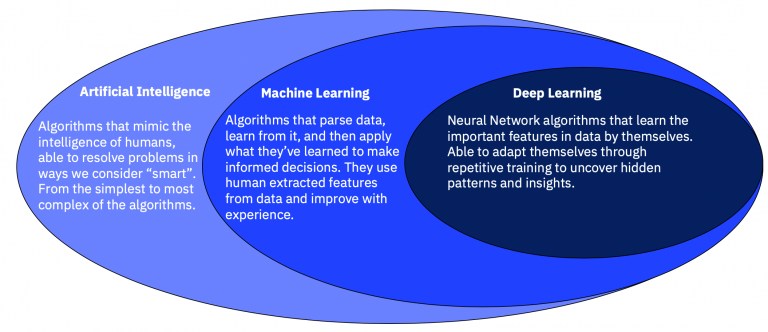
\includegraphics[width=12cm]{rodrigo1-768x332.png}
	\caption{From \href{https://www.ibm.com/blogs/systems/ai-machine-learning-and-deep-learning-whats-the-difference/}{AI, machine learning and deep learning: What’s the difference?} by Rodrigo Ceron.}
	\label{aimldl}
\end{figure}

\section{\label{sec:terraform}Collecting Infrastructure Code as a Data Source}

\justifying
Some level of familiarity on the reader's part with \href{https://www.terraform.io/intro/index.html}{Terraform} and
by extension, \href{https://learn.hashicorp.com/tutorials/terraform/infrastructure-as-code}{Infrastructure as Code} is assumed.
\vspace{2mm}

\justifying
Terraform users create files that define network infrastructure. When this infrastructure is deployed via Terraform, a state file is created to keep track of the current deployment. This state file is essentially graph structured data. We can export this graph data from the actual (or planned) state and ingest this
with our deep learning pipeline.

\subsection{\label{sec:collect}The Data Collection Process}

\justifying
A tool for gathering and uploading from data sources is used to send relevant data
from various sources to a storage bucket in Google Cloud. Raw data is processed and tagged with a UUID as a unique key to associate data with it's source. The
source code for this Python tool is \href{https://github.com/devsecfranklin/model-graph-neural-net/tree/main/src}{available in the Github repository for this project}.
\vspace{2mm}

\justifying
Identifying and
versioning data as we would any other code or documentation artifact eases the
burden of handling our data and allows us to more easily work with larger data sets.
\vspace{2mm}

\justifying
While the collection process is relatively straight forward to implement and maintain for this project on a small hobbyist/researcher scale, going forward it would make more sense to use a \href{https://github.com/iterative/dvc}{community supported framework such as dvc} to leverage the efforts of folks doing similar work.

\section{\label{sec:iacdata}Using Infrastructure Code as Data}

\justifying
Once a Terraform code base has been initialized, the user has the option to generate
a directed graph of the infrastructure using Dot. Dot is \href{https://graphviz.org/doc/info/lang.html}{a language used to describe graphs}. Consider the following declaration of a
Cloud Function for Google Cloud.

\begin{mybox}{\thetcbcounter: Terraform Declaration Example}
    \lstinputlisting{code/main.tf}
\end{mybox}

\justifying
\href{https://graphviz.org/}{Graphviz is open source graph visualization software}. Graph visualization is a way
of representing structural information as diagrams of abstract graphs and networks.
Conversion of Terraform HCL to a directed graph representation is trivial thanks to Graphviz and Dot. It is possible to reproduce the
digraph displayed in figure \ref{pygraph} \href{https://github.com/devsecfranklin/model-graph-neural-net/blob/main/paper/code/gen_graph.sh}{using the shell script provided}.

\justifying
\begin{figure}[H]
	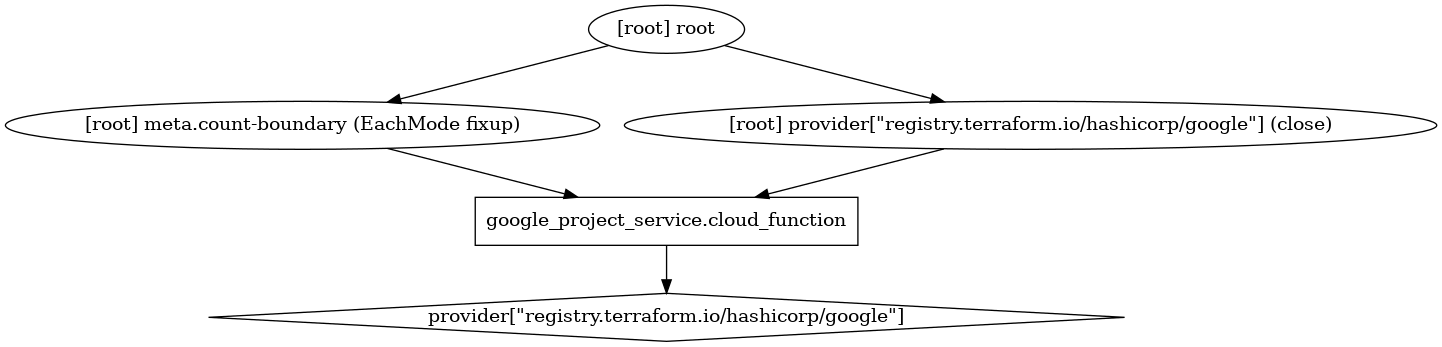
\includegraphics[width=12cm]{graph.png}
	\caption{DOT output from Terraform Files as a digraph}
	\label{pygraph}
\end{figure}

\section{\label{sec:collection}Data Collection}

\justifying
Run a small tool to collect data and pass results to a Google Cloud storage bucket.

\subsection{\label{sec:conversion}Conversion of a Digraph}

\justifying
Once our Terraform infrastructure has been output as a directed graph, we need to bring it in to Python so we can
perform operations on it. To run Terraform commands in an automated fashion,
the \href{https://pypi.org/project/python-terraform/}{python-terraform module} is used.
\vspace{2mm}

\justifying
Directed graphs are ingested into Python as an object using the \href{https://pypi.org/project/networkx/}{networkx module}. Now we are prepared
to perform computational operations on the digraph.
\vspace{2mm}

\justifying
\begin{figure}[H]
    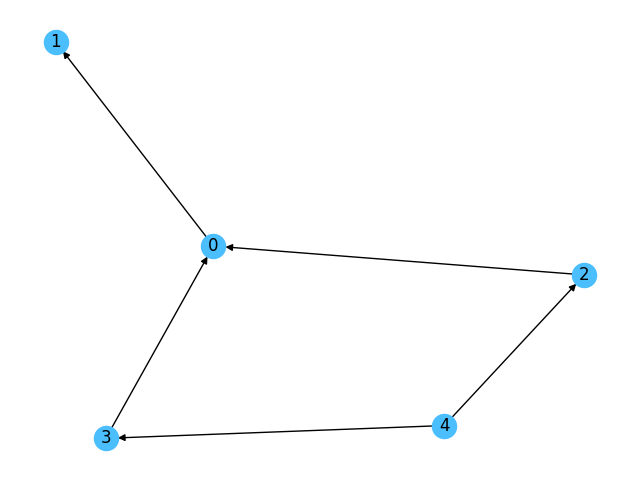
\includegraphics[width=12cm]{graph3.png}
    \caption{Directed graph as ingested by Networx}
    \label{digraph}
\end{figure}

\justifying
Note that new numerical labels are displayed in place of the original labels. These are
stored in the node objects in case we need them later. The root node of the adjacency matrix is labeled
as the 0th element in the graph. Also of note is that the graphs displayed in figure \ref{pygraph} and figure \ref{digraph} can be described as \href{https://en.wikipedia.org/wiki/Graph\_isomorphism}{isomorphic}.
\vspace{2mm}

\justifying
Cleaning data using the \href{}{pyjanitor module}.
\vspace{2mm}

\subsection{\label{sec:adjacency}The Adjacency Matrix}

\justifying
The adjacency matrix is a mathematical representation of our graph. The nodes are represented in a
columnar format known as a matrix. Continuing with our previous example, the representation of our

Add the identity matrix to the adjacency matrix using an update rule.
The goal is to prevent the central node from being excluded. Doing this without increasing the scale requires something like multiplication by the inverse of the degree matrix, aka ``mean pooling''. The
most popular graph convolutional layer is the GCN update rule. We will not be able to attach complex features to the edges.

\subsection{\label{sec:embedding}Node Embedding}

\justifying
Assigning weights and features to the edges of the graph. Labeling.

Attach feature vectors to nodes.

Compute arbitrary message vectors between neighbor nodes.

\subsection{\label{sec:conv}Convolutional Layers}

\section{\label{sec:visualization}Data Visaulization}

\section{\label{sec:reading}Resources}

\justifying
Here is a quick list of things that I found interesting and relevant.

\begin{raggedright}
	\begin{enumerate}
		\item There is an excellent \href{https://www.youtube.com/watch?v=8owQBFAHw7E}{talk on YouTube by Petar Veličković}, a research scientist at \href{https://deepmind.com/about}{DeepMind}.
		\item The \href{https://github.com/tkipf/gcn}{Kipf and Welling GCN repo on GitHub}.
    \end{enumerate}
\end{raggedright}
\vspace{2mm}

\clearpage
\begin{versionhistory}
	\vhEntry{v0.1}{Nov. 20th, 2021}{Franklin Diaz}{Initial Draft}
\end{versionhistory}
\nocite{*}
\bibliographystyle{plain}
\bibliography{mybib.bib}

\end{document}
